\chapter{Results and Discussion}
\label{ch:4}
\noindent

\section{Computation Times of Fragmentation Expansion}

Computation times present a significant bottleneck for this approach. 
The \texttt{mod} framework, while powerful in generating comprehensive reaction networks, 
prioritizes flexibility and completeness over computational efficiency. 
Combined with the combinatorial explosion of possible fragments and parent molecules, 
runtime becomes prohibitive as the number of fragmentation rules increases. 
Since only a subset of known rules were applied in this study, 
computation times per molecule will rise substantially as additional rules are incorporated, 
making further optimization necessary to ensure the feasibility of this approach at scale.

\subsection{Visualization of Computation Times}

A regression analysis was performed to model the relationship between molecular complexity and computation time.
The analysis assumes:
\begin{itemize}[noitemsep,topsep=0pt]
    %\item Linearity of the relationship
    \item Homoscedasticity of residuals
    \item Independence of residual observations
    \item Normality of residual distribution
\end{itemize}

In Figure \ref{fig:mod-time-regres}, the regression results are visualized, 
showing a positive correlation between molecular complexity and computation time, 
but also show a large variance in computation times for molecules of similar complexity.
Note that the threshold of 40 seconds was chosen arbitrarily to exclude trivial expansions.

\begin{figure}[ht]
    \centering
    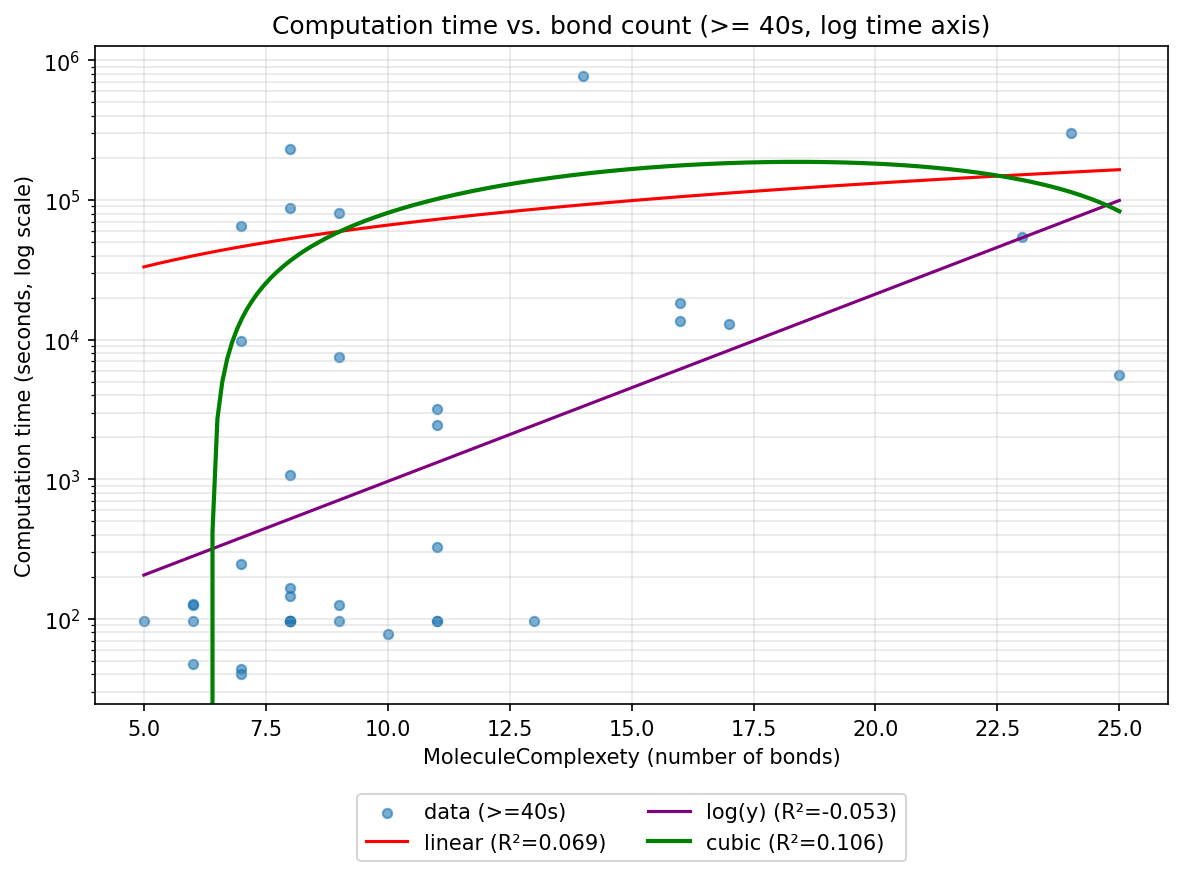
\includegraphics[width=0.8\linewidth]{time_vs_complexity_logy_over40.png}
    \caption[Fragmentation Computation Times]{
        Regression of Computation time, excluding molecules that had trival expansions (time $< 40$s).
        The plot shows a positive correlation between molecular complexity and computation time,
        but also a large variance in computation times for molecules of similar complexity.
        }
    \label{fig:mod-time-regres}
\end{figure}

So while there is a general trend of increasing computation time with molecular complexity,
the large variance suggests that other factors, 
such as specific structural features or the particular fragmentation pathways available, also play a significant role in determining computation time. 
This highlights the need for further optimization.

% model size 
\subsection{Data Splits}

The dataset was partitioned in two stages into training, validation, and test subsets. 
In the first stage, the full set of molecule--spectrum pairs was divided into 
an 80\% training portion and a 20\% test portion. 
In the second stage, the initial training portion was further split into 70\% training and 30\% validation. 
This results in a final distribution of 56\% training data, 24\% validation data, 
and 20\% test data relative to the original dataset.

These ratios were chosen as a pragmatic trade-off between model development and robust evaluation. 
The $80/20$ split keeps a sufficiently large hold-out test set for a meaningful final performance estimate, 
while still reserving most samples for development. Splitting the development portion into $70/30$ then 
provides enough training data for parameter learning and enough validation data for stable model selection 
and hyperparameter tuning.

This splitting strategy serves two purposes. 
First, it preserves a dedicated hold-out test set that is never used during model development 
and is therefore reserved for the final evaluation. 
Second, it provides a separate validation set for model selection, hyperparameter tuning, 
and intermediate performance monitoring. 
In this way, the validation set supports iterative model development, 
while the test set remains an unbiased reference for the final assessment.

All splits are generated with a fixed random seed (\texttt{random\_state=42}) to ensure reproducibility. 
At the same time, the implementation uses \texttt{shuffle=False}, so the split is deterministic and 
preserves the original order of the dataset rather than randomly permuting the samples beforehand. 
This design choice has to be interpreted carefully. 
On the one hand, it guarantees that repeated runs use exactly the same partitioning. 
On the other hand, if the original ordering of molecules is not random, 
the resulting subsets may differ systematically in composition. 
The reported results should therefore be understood with this deterministic split procedure in mind.

An additional technical constraint concerns the fragment representation. 
The fragment vocabulary is constructed only from the training set 
and then reused unchanged for the validation and test sets. 
This ensures that the dimensionality of fragment-based model components 
remains fixed across all stages of training and evaluation. 
It also prevents information leakage from validation or test data into the feature space used during training. 
In practical terms, this means that fragment identifiers available during evaluation are restricted to 
those observed in the training data, which is consistent with a realistic supervised learning setting.

Overall, the chosen split strategy provides a clear separation between model fitting, model selection, 
and final evaluation, while maintaining a consistent fragment representation across all subsets. 
At the same time, the use of a deterministic non-shuffled split should be considered 
when interpreting the generality of the reported results.


\section{Evaluation of Fragment Prediction}

The evaluation reveals a mixed but informative picture of the proposed framework. 
On the one hand, the model learns a usable mapping between molecular structures and spectra in both directions. 
On the other hand, the fragment-aware components do 
not currently provide a clear empirical advantage over simpler ablated variants. 
The strongest positive result instead arises from the reranking stage, 
which substantially improves retrieval quality.
To isolate the contribution of individual components, this section includes an \emph{ablation study}
comparing the full model against no-fragments, no-derivation-tree, and no-reranking variants.
The paired randomization tests underlying this comparison did not yield statistically significant
differences for any of the pairwise contrasts, with all p-values exceeding $0.05$.

\begin{figure}[H]
    \centering
    \includesvg[width=0.8\linewidth]{fig-tikz/cosine_mrr.svg}
    \caption[Cosine similarity and MRR for ablation variants]{
        Ablation of three pipeline components (fragments, derivation tree, and reranker) against the full model. 
        Cosine similarity measures how similar the query is to the correct target, averaged over all queries; 
        MRR is the mean reciprocal rank of the ground-truth target. 
        Error bars show $95\%$ bootstrap confidence intervals (5000 query resamples). 
        Brackets indicate pairwise p-values from paired randomization tests 
        %on per-query differences (10,000 sign flips), 
        computed separately for each metric. 
        Cosine similarity remains nearly constant across variants ($\approx 0.43$), 
        while MRR decreases from $0.24$ to $0.10$ when reranking is removed. 
        Since all confidence intervals overlap and all pairwise p-values exceed $0.05$, 
        these differences should be interpreted as suggestive rather than statistically established.
        }
    \label{fig:cosine-mrr}
\end{figure}

In this ablation study, with respect to the forward task, 
all evaluated variants achieve very similar cosine similarity values. 
The full model reaches a mean cosine similarity of $0.4316$, while the no-fragments 
and no-derivation-tree ablations achieve $0.4327$ and $0.4322$, respectively. Which is visible in \Cref{fig:cosine-mrr}.
These differences are extremely small and indicate that the forward reconstruction quality is 
largely insensitive to the inclusion or removal of the current fragment-aware branch. 
In practical terms, the molecular encoder appears to capture most of the predictive signal required 
for the structure-to-spectrum task, while the fragment representation 
does not yet provide an additional measurable benefit.

The retrieval results are more informative. As shown in Figure \ref{fig:recall-at-k}, for the full model, 
Recall@1 is $0.091$, Recall@5 is $0.318$, Recall@10 is $0.500$, and Recall@20 is $0.864$, 
with a mean reciprocal rank (MRR) of $0.243$. This shows that the correct molecule is frequently brought 
into the top portion of the ranked candidate list, although top-1 identification remains limited. 
The model therefore behaves more like a candidate narrowing system than a reliable single-shot identifier, 
which is still useful in practical structure elucidation workflows.

\begin{figure}[H]
    \centering
    \includesvg[width=0.8\linewidth]{fig-tikz/recall_at_k.svg}
    \caption[Recall@k for ablation variants]{
        Recall@k for $k = 1, \ldots, 20$ across the full retrieval model and three ablated variants. 
        Shaded bands show 95\% bootstrap confidence intervals over queries. 
        The full model and the \texttt{no fragments}~/~\texttt{no derivation tree} variants 
        cluster together across the full $k$ range, 
        while the \texttt{no reranking} variant trails the others at every $k$, 
        with the largest gap at small $k$ and gradual closure toward $k = 20$.
    }
    \label{fig:recall-at-k}
\end{figure}

The clearest effect in the evaluation is observed for the reranking stage. 
Removing reranking leaves the forward cosine similarity unchanged, as expected, 
but substantially reduces retrieval quality. Recall@5 drops from $0.318$ to $0.091$, 
Recall@10 from $0.500$ to $0.227$, Recall@20 from $0.864$ to $0.409$, and MRR from $0.243$ to $0.103$. 
This demonstrates that much of the retrieval benefit of 
the framework arises from combining latent-space retrieval with forward-model-based rescoring. 
In this sense, the present implementation benefits more from the interaction between the forward 
and backward branches than from the fragment-aware representation itself.

By contrast, the fragment-related ablations do not support a strong performance claim. 
The no-fragments variant performs slightly better than the full model on cosine similarity and Recall@5, 
but slightly worse on Recall@10, Recall@20, and MRR. Similarly, the no-derivation-tree variant is 
highly competitive and even slightly exceeds the full model on Recall@5 and MRR. 
These results suggest that the fragment branch, in its current form, 
is not yet contributing a robust and clearly positive signal. 
At present, it appears to be largely redundant with the molecular representation, 
and may in some cases introduce noise rather than useful structure.

This conclusion should, however, be interpreted cautiously. 
The test set contains only $22$ queries, so recall values change in increments of approximately $0.045$. 
Consequently, differences between variants often reflect only one or two queries. 
Query-level paired analyses confirm that the differences between the full model 
and the no-fragments ablation are not statistically convincing for the main metrics, 
whereas the benefit of reranking is much more substantial. 
The present evaluation therefore provides stronger support for the usefulness of reranking than 
for the effectiveness of the fragment-aware branch.

Overall, the results show that the proposed bidirectional framework is functional and 
that reranking substantially improves retrieval performance. 
However, they also indicate that the current fragment integration does not yet realize its intended benefit. 
The main contribution of the present work is therefore not the demonstration of a clear 
performance gain from fragment augmentation, 
but rather the establishment of a fragment-augmented bidirectional framework whose strengths, weaknesses, 
and failure modes can be analyzed systematically. 
This in turn provides a concrete basis for future work aimed at improving the informativeness 
and integration of fragment-level intermediate representations.

%\section{Forward Model Evaluation}
%\subsection{Spectral Similarity and Fragment Prediction}

%\section{Backward Model Evaluation}
%\subsection{Structure Reconstruction and Validity}
%\subsection{Reward Convergence and Exploration Efficiency}

%\section{Comparison with Baseline Models}
%CFM-ID, 
%
%MSNovelist (https://doi.org/10.1038/s41592-022-01486-3), 
%
%MassGenie (https://doi.org/10.3390/biom11121793) ...



%\chapter{Discussion}
%\label{ch:5}

%\section{Benefits of Fragment-Aware Modeling}
%How fragments improve interpretability.

\section{Challenges}
The thesis is shaped by several interconnected challenges. 

\textbf{First}, fragmentation must be represented in a way that is 
simultaneously chemically meaningful and useful for machine learning. 

\textbf{Second}, explicit fragment generation leads to 
a \emph{combinatorial explosion} of candidate structures and limits the practical scale of the approach. 

\textbf{Third}, the absence of unique \emph{ground-truth fragmentation trees} makes 
fragment-level supervision inherently \emph{ambiguous}. 

\textbf{Fourth}, bidirectional learning introduces \emph{competing objectives}, 
since forward spectrum reconstruction and backward structure retrieval do not necessarily favor the same latent 
representation. 

\textbf{Fifth}, evaluation is intrinsically multi-dimensional, requiring predictive, retrieval-based, 
and interpretability-oriented criteria. 

Finally and \textbf{sixth}, the empirical contribution of fragment-aware intermediate representations remains difficult 
to establish conclusively, especially under \emph{small-sample} conditions and in the presence of strong baseline 
signals from the molecular encoder alone.


%\section{potential improvements}
%speed up graph transformation, especially predicates
%trivial, scoping: use one class of molecules, a diverse set of molecules is naturally more difficult to model.